\documentclass[journal,12pt,twocolumn]{IEEEtran}
\usepackage[utf8]{inputenc}
\usepackage{amssymb}
\usepackage{setspace}
\usepackage{gensymb}
\singlespacing
\usepackage[mathscr]{euscript}
\usepackage{textgreek}
\usepackage{textcomp}
\usepackage{amsmath}
\numberwithin{equation}{section}
\usepackage{mathrsfs}
\usepackage{txfonts}
\usepackage{stfloats}
\usepackage{bm}
\usepackage{cite}
\usepackage{hyperref}
\usepackage{cases}
\usepackage{subfig}
\usepackage{graphicx}
\usepackage{circuitikz}
\usepackage{tikz} 
\usetikzlibrary{karnaugh}
\usepackage{listings}
\usepackage{amsfonts}
\usepackage{longtable}
\usepackage{multirow}
\usepackage{tcolorbox}
\usepackage{geometry}
\usepackage{tikz}
\usetikzlibrary{shapes.gates.logic.US}
\usetikzlibrary{circuits.ee.IEC}


\geometry{
 a4paper,
 total={170mm,257mm},
 left=20mm,
 top=20mm,
 }
\usepackage{listings}
\lstset{
frame=single, 
breaklines=true,
columns=fullflexible
}

\def\putbox#1#2#3{\makebox[0in][l]{\makebox[#1][l]{}\raisebox{\baselineskip}[0in][0in]{\raisebox{#2}[0in][0in]{#3}}}}
     \def\rightbox#1{\makebox[0in][r]{#1}}
     \def\centbox#1{\makebox[0in]{#1}}
     \def\topbox#1{\raisebox{-\baselineskip}[0in][0in]{#1}}
     \def\midbox#1{\raisebox{-0.5\baselineskip}[0in][0in]{#1}}
\vspace{3cm}

\usepackage{karnaugh-map}
\usepackage{hyperref}

\renewcommand\thesection{\arabic{section}}
\renewcommand\thesubsection{\thesection.\arabic{subsection}}
\renewcommand\thesubsubsection{\thesubsection.\arabic{subsubsection}}

\renewcommand\thesectiondis{\arabic{section}}
\renewcommand\thesubsectiondis{\thesectiondis.\arabic{subsection}}
\renewcommand\thesubsubsectiondis{\thesubsectiondis.\arabic{subsubsection}}

\title{FPGA Lab Assignment 1}
\author{EE20MTECH14016 - Pulkit Saxena}

\begin{document}

\maketitle

\section{Question}

[CBSE 2019 Q6 (a)] State any one Distributive Law of Boolean Algebra and verify it using truth table.

\section{Solution}
Distributive Law is as follows:-
\begin{align}
 A.(B+C) \\
= A.B+A.C
\end{align}

\section{Truth Table}
Verification of the above stated distributive law using truth table is as follows.
\medskip

    \centering
          \begin{tabular}{|c|c|c|c|c|c|c|c|}
            \hline
            A & B & C & B+C & A.(B+C) & A.B & A.C & A.B+A.C \\
            \hline
            0 & 0 & 0 & 0 & 0 & 0 & 0 & 0\\
            \hline
             0 & 0 & 1 & 1 & 0 & 0 & 0 & 0\\
            \hline
             0 & 1 & 0 & 1 & 0 & 0 & 0 & 0\\
            \hline
             0 & 1 & 1 & 1 & 0 & 0 & 0 & 0\\
            \hline
            1 & 0 & 0 & 0 & 0 & 0 & 0 & 0\\
            \hline
            1 & 0 & 1 & 1 & 1 & 0 & 1 & 1\\
            \hline
            1 & 1 & 0 & 1 & 1 & 1 & 0 & 1\\
            \hline
            1 & 1 & 1 & 1 & 1 & 1 & 1 & 1\\
            \hline
            
        \end{tabular}
        \begin{align}
		 A.(B+C) = A.B+A.C
		\end{align}
     

\section{Karnaugh Map}


\begin{figure}[h!]
    \centering
    \begin{karnaugh-map}[4][2][1][][]
        
        \minterms{5,6,7}
        \maxterms{0,1,2,3,4}
        \implicant{5}{7}
        \implicant{7}{6}
        \draw[color=black, ultra thin] (0, 2) --
        node [pos=0.7, above right, anchor=south west] {$BC$} % Y label
        node [pos=0.7, below left, anchor=north east] {$A$} % X label
        ++(135:1);
        
    \end{karnaugh-map}
    \caption{K-Map for $A.B + A.C$}
    \label{fig:kmap}
\end{figure}


\section{Circuit Diagram(Inplementation using NAND gates)}


    \begin{center}
    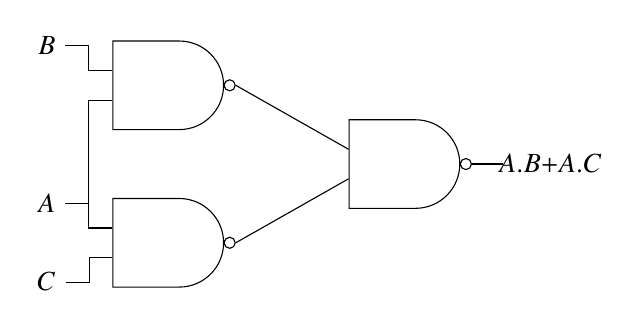
\begin{tikzpicture}[ ]
    
    \node (C) at (0,0) {$C$};
    \node (A) at (0,1) {$A$};
    \node (B) at (0,3) {$B$};
    \node[nand gate US, minimum size=32pt, draw] at (1.5,0.5) (NAnd) {};
    \node[nand gate US, minimum size=32pt, draw] at (1.5,2.5) (NAnd1) {};
    \node[nand gate US, minimum size=32pt, draw] at (4.5,1.5) (NAnd2) {};
    \draw (C.east) - ++(right:3mm) |- (NAnd.input 2);
    \draw (A.east) - ++(right:3mm) |- (NAnd.input 1);
    \draw (B.east) - ++(right:3mm) |- (NAnd1.input 1);
    \draw (A.east) - ++(right:3mm) |- (NAnd1.input 2);
    %\draw (3.85,1.5) -- (3,1.5);
    %\draw (3,0.5) -- (3,2.5);
    \draw (NAnd.output) -- (NAnd2.input 2);
    \draw (NAnd1.output) -- (NAnd2.input 1);
    \node (z) at ($(NAnd2) + (1.9,0)$) {$A. B$+$A .C$};
    \draw (5.4,1.5) -- (5.8,1.5);
    
    \end{tikzpicture}
    \end{center}

\end{document}





